\documentclass[10pt,letterpaper]{article}

\usepackage{cogsci}
\cogscifinalcopy % Uncomment this line for the final submission 
\usepackage[hidelinks]{hyperref}
\usepackage{hyperref}
\usepackage{graphicx}
\usepackage{caption}
\usepackage{subcaption}
\usepackage{pslatex}
\usepackage{apacite}
\usepackage{natbib}
\usepackage{amsmath}
\usepackage{float} % Roger Levy added this and changed figure/table
                   % placement to [H] for conformity to Word template,
                   % though floating tables and figures to top is
                   % still generally recommended!
\usepackage{lipsum}
%\usepackage[none]{hyphenat} % Sometimes it can be useful to turn off
%hyphenation for purposes such as spell checking of the resulting
%PDF.  Uncomment this block to turn off hyphenation.

%\setlength\titlebox{4.5cm}
% You can expand the titlebox if you need extra space
% to show all the authors. Please do not make the titlebox
% smaller than 4.5cm (the original size).
%%If you do, we reserve the right to require you to change it back in
%%the camera-ready version, which could interfere with the timely
%%appearance of your paper in the Proceedings.

\usepackage{setspace} % for \onehalfspacing and \singlespacing macros
\onehalfspacing 
\usepackage{etoolbox}
\AtBeginEnvironment{quote}{\singlespacing\small}

\title{How do disparities reproduce themselves? ``Ground truth'' inference from utility-maximizing agent's sampling behavior}
 
\author{{\large \bf Yuan Meng} \\ \href{mailto:yuan_meng@berkeley.edu}{\texttt{yuan\_meng@berkeley.edu}} \\ Department of Psychology \\ University of California, Berkeley
     \And {\large \bf Fei Xu} \\ \href{mailto:fei_xu@berkeley.edu}{\texttt{fei\_xu@berkeley.edu}} \\ Department of Psychology \\ University of California, Berkeley
    }


\begin{document}

\maketitle

\begin{abstract}
In an ideal world, evidence of disparities motivates people to fight them; in reality, disparities often ``reproduce'' themselves. Upon seeing the police stopping some groups at higher rates, people may believe members of these groups are more prone to crime and therefore seek more punitive measures against them. In this paper, we argue that even without stereotypic associations linking some groups with crime, people may still reproduce observed disparities via rational inference: Assuming an agent is knowledgeable about a target trait's ``hit rates'' in different groups and acts to maximize the expected utility of checking, you may infer that groups checked more often have higher hit rates. In Experiment 1, this ``Na\"ive Utility Calculus'' successfully captured how people inferred the hit rate in a population based on how often an agent sampled from it (``check rate''). In Experiment 2, when hit rates in the samples were revealed, people predominantly relied on this new information more heavily than the agent's check rates. Our work both provided a novel explanation for why people reproduce disparities and a potential intervention to combat such a tendency.

\textbf{Keywords:} social cognition; disparities; theory of mind; computational modeling

\end{abstract}

\section{Introduction}
In Oakland, California, around 60\% of the police stops between 2013 and 2014 were of African Americans, who only make up about 28\% of the local population and were no more likely than members of other races to carry contraband \citep*{hetey2016data}. Not only does intense proactive policing tend to induce psychological stress and future crimes in the African American community \citep*{del2019criminogenic}, it's also the first step towards disparities in areas with more dire consequences, such as arrests and incarceration. As scientists and educators, what can we do to help combat racial disparities in proactive policing?

Perhaps if people saw what we saw, they would be eager to end racial disparities. However, numbers don't always speak for themselves: Evidence of disparities often leads people to support the very system that has created them in the first place \citep{hetey2018numbers}. For instance, when presented with a ``Blacker'' prison compared to a ``less Black'' one (45\% \emph{vs.} 25\% inmates were African Americans), White voters became more supportive of laws that severely punish repeated offenders \citep{hetey2014racial}. Why would people support laws that may intensify racial disparities after being made more aware of their existence? Hetey and Eberhardt (2014, 2018) argued that this paradox could be explained by stereotypic associations linking Blacks with crime: A Blacker prison made people more fearful of crime and the fear prompted them to support stricter criminal law. 

Are pre-existing stereotypes such as the ``Black-crime association'' necessary for observers to reproduce disparities? Imagine, as a new quality inspector at a factory, you shadowed the most experienced inspector on your first day there. They checked 7 out of every 10 X products and only 3 out every 10 Y products. Inspecting a product incurs a small cost every time but catching a defective one is far more rewarding. When it's your turn, would you check X or Y more often? If your answer is ``X'', is it because you have stereotypic associations linking it with low quality? This explanation is unlikely since you've only just seen these products. Alternatively, your preference may be a result of \emph{rational inference}: Assuming the inspector is knowledgeable about product quality and acts to maximize the expected utility of checking (the expected reward from finding defective products minus the total cost of checking), it only makes sense if X has a higher defect rate than Y---so you should also check X more often, just like your predecessor did. This kind of \emph{Na\"ive Utility Calculus} \citep*[NUC,][]{jara2016naive} explains how we might end up reproducing disparities we observe without having any stereotypes from the get-go.

\subsection{Inferring ``ground truth'' from sampling processes}
It's not a new idea that sampling behavior is a window into an intentional agent's preference. Even young children \citep*{kushnir2010young} and infants \citep*{wellman2016infants} understand that a person selecting rare toys at a disproportionately high rate prefers these toys and will choose the same type in the future. It's also been proposed that such inferences arrive from a \emph{principle of efficiency} \citep*{jara2018sensitivity}: A utility-maximizing agent wouldn't go out of their way to seek out the rarer option if they didn't like it better.

The police scenario differs from previous studies in that we care \emph{not} about how people use sampling to infer others' preference but some ``ground truth'' about the world. To our best knowledge, only one study \citep*{gweon2010infants} has looked at ground truth inference from non-random sampling. In their study, infants had to infer was whether a property (squeaking) found in one category (blue balls) extended to another (yellow balls). When most balls were yellow but the experimenter only sampled blue balls which all squeaked, infants didn't expect yellow balls to also squeak (\emph{``If yellow balls also squeak, why didn't she show me?''}). 

Ground truth inference in our study goes beyond binary: Rather than whether a trait extends to a group, people must infer the prevalence of that trait. After all, members of all races commit crime but what observers believe drives the police's sampling behavior is the magnitude of crime rates. Furthermore, infants in Gweon et al.'s (2010) study had to simultaneously infer whether the experimenter was sampling from all balls or just squeaking balls. This joint inference captures observers' uncertainty about both the police's intention and knowledge. However, before factoring in the agent's intention, we want to first establish whether people can make accurate inference about ``crime rates'' based on sampling. We made it clear that the agent is cost-effective and knowledgeable about true ``crime rates'' in different groups. In the future, it's worth exploring joint mental state/ground truth inference as a model of how people learn from a rational agent's sampling behavior and also a potential anti-bias intervention.

By viewing the reproduction of disparities from a rational perspective, by no means do we wish to ``rationalize'' it or downplay the role of stereotypes discussed in a vast body of literature \citep*[e.g.,][]{eberhardt2004seeing,payne2001prejudice}. Rather, what we are ultimately searching for is an effective way to fight disparities and if we find that rational inference alone has the power to reproduce disparities, we need further measures than just doing away with stereotypes.

\subsection{Study overview}
To capture key elements of proactive policing without evoking pre-existing racial stereotypes, we designed a novel arcade game called the ``Golden Ticket'' (Figure \ref{fig:example}). In this game, a robot chicken lays one egg at a time, which is either empty or has a golden ticket that can be redeemed for a grand prize. Each egg costs a token and tokens are expensive and come in limited quantities. Players can pass on eggs that they don't want to buy. This game is designed to simulate real-life police encounters. A robot chicken and the eggs it lays are akin to a social group and members of that group and the player symbolizes the police officer. Winning a golden ticket and catching a criminal are both highly rewarding yet checking incurs a cost every time, be it a token or time and energy. Each chicken has a fixed \emph{``hit rate''} (the probability of laying an egg that has a golden ticket) known to an experienced player Alex. Alex also doesn't spend tokens unnecessarily. Participants watched Alex play a series of robot chicken. After each, they were asked to infer the chicken's hit rate and indicate whether they wanted to buy a new egg from it.

\begin{figure}[t]
  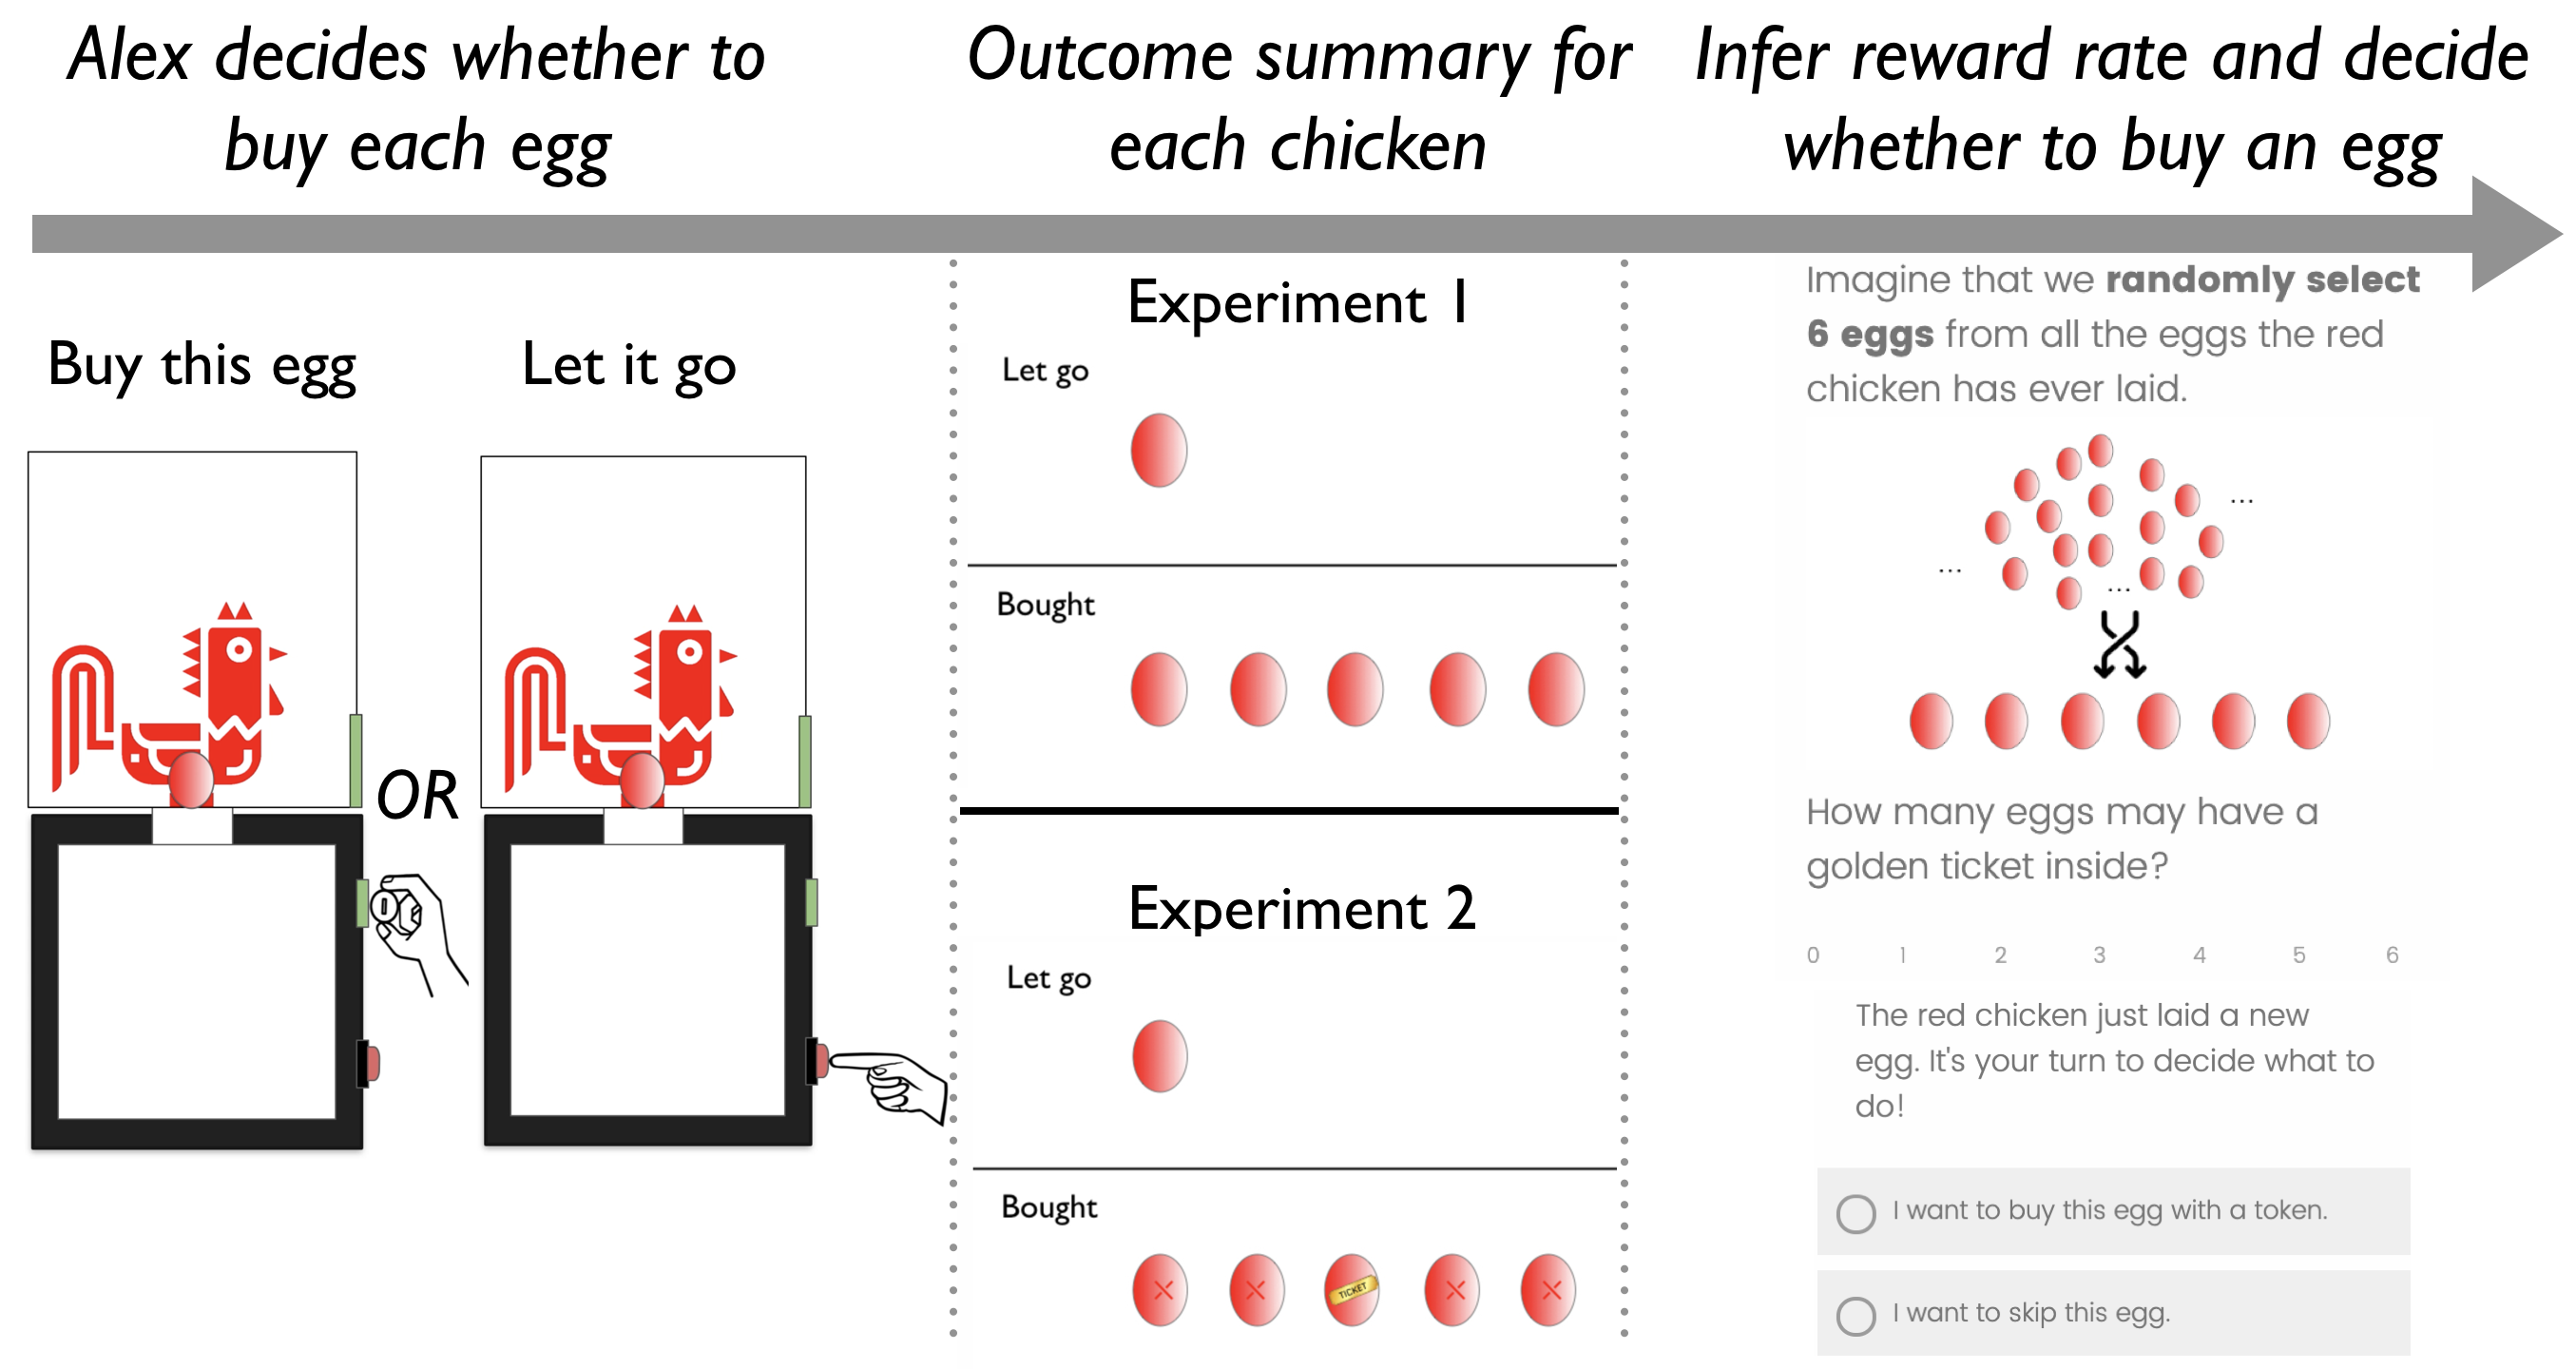
\includegraphics[width=\linewidth]{example.png}
  \caption{The Golden Ticket game: A robot chicken laid a total of 6 eggs one at a time. Alex, the best player who knew every chicken's hit rate and refrained from unnecessary purchase, decided whether to buy each egg or let it go. In Experiment 1, participants only saw how many eggs Alex bought but not the content of the eggs. In Experiment 2, Alex opened the eggs they bought, revealing which ones had tickets and which ones were empty. At the end of each trial, participants were asked to estimate the hit rate of the robot chicken and indicate whether they want to buy a new egg laid by this chicken.} 
  \label{fig:example}
\end{figure}

In Experiment 1, the eggs' content was not revealed. We looked at whether participants could infer hit rates based on \emph{``check rates''} (the probability that Alex buys an egg from a chicken) alone. Their inferences were compared to predictions generated by a Na\"ive Utility Calculus model. In Experiment 2, Alex opened the eggs after each round. We examined whether participants used both the hit rate and the check rate in the sample to infer the true hit rate in the population or if they relied on one source of information. We created three computational models to compare against human performance, each corresponding to an aforementioned possibility (hit rate only, check rate only, check + hit rates).

\section{Computational Modeling}

\begin{figure}[t]
  \centering
  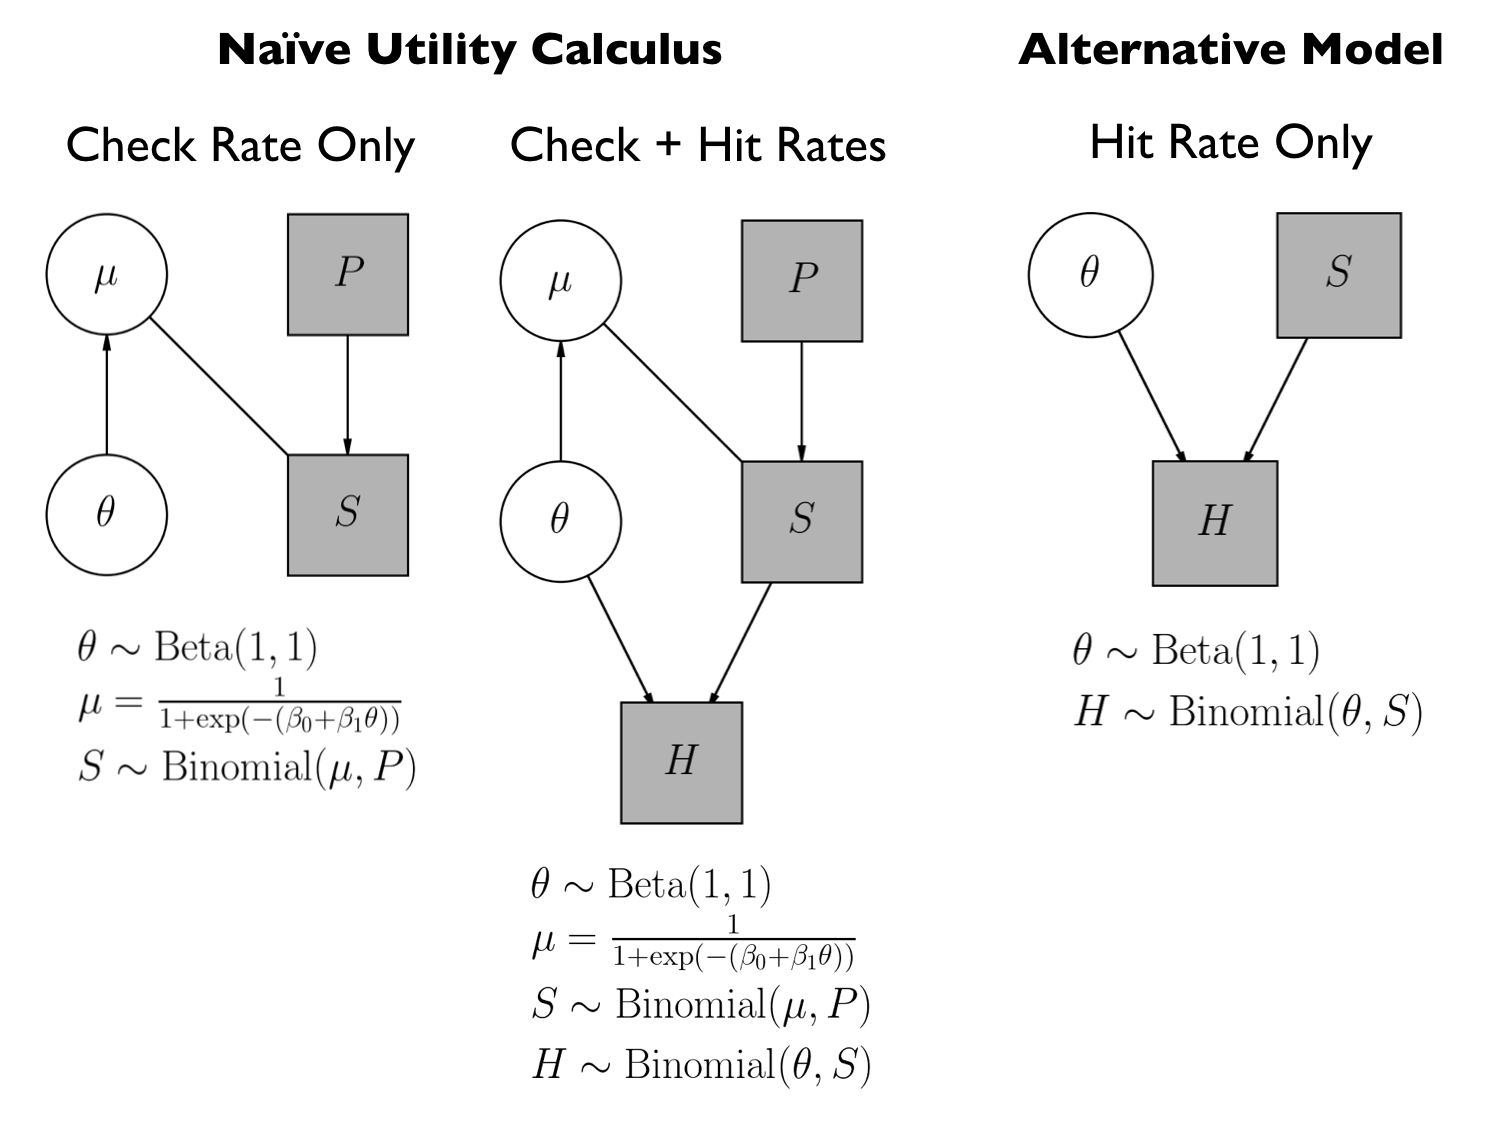
\includegraphics[width=\linewidth]{model.png}
  \caption{Computational models of hit rate inference. In the two Na\"ive Utility Calculus (NUC) models, the check rate $\mu$ is inferred from the number of eggs Alex bought ($S$) out of the number of eggs a chicken laid ($P$). $\mu$ is linked to the true hit rate $\theta$ via a logistic function, whose intercept $\beta_0$ and slope $\beta_1$ are estimated from participants' inferred hit rates and purchase decisions. In Experiment 1, $\theta$ can only be inferred from $\mu$. In Experiment 2, $\theta$ can be simultaneously inferred from $\mu$ and the number of eggs with tickets ($H$) out of $P$. Alternatively, people may ignore $\mu$ and assume that the observed hit rate is the true hit rate, in which case ``hit rate only'' model captures their inference.}
  \label{fig:models}
\end{figure}

\subsection{Na\"ive Utility Calculus models}
We created computational models based on the Na\"ive Utility Calculus (NUC) \citep{jara2016naive} to predict how learners infer each chicken's hit rate from Alex's check rate. The key assumption is that Alex maximizes the expected rewards of winning golden tickets relative to the total costs of buying eggs. Suppose each ticket has a value of $V$, each token costs $C$, and the true hit rate of a chicken is $\theta$, then the expected utility of buying an egg from a given chicken is:

\begin{equation} \label{eq1}
\mathrm{E}[U(buy)] = V\theta - C
\end{equation}

The higher the expected utility $\mathrm{E}[U(buy)]$, the more likely that Alex will buy an egg, hence the higher the check rate $\mu$. We assume that Alex's choice behavior follows a softmax choice rule \citep{sutton998}. In the case of binary choices, the softmax function becomes the logistic function:

\begin{equation} \label{eq2}
\mu = \frac{1}{1 + \exp (-\mathrm{E}[U(buy)])/\tau}
\end{equation}

where $\tau$ is a temperature parameter controlling the level of stochasticity in Alex's decisions. When $\tau \to 0$, Alex will always buy an egg if $\mathrm{E}[U(buy)] > 0$; when $\tau \to \infty$, Alex just randomly decides between buying an egg and letting it go. 

The three free parameters $V$, $C$, and $\tau$ can be absorbed into the slope $\beta_1 = V/\tau$ and the intercept $\beta_0 = -C/\tau$ of the logistic function in Equation \ref{eq2}, which then becomes:

\begin{equation} \label{eq3}
\mu = \frac{1}{1 + \exp (-(\beta_0 + \beta_1\theta))}
\end{equation} 

We can estimate $\beta_0$ and $\beta_1$ from participants' inferred hit rates and subsequent purchase decisions. Plugging the estimates back in Equation \ref{eq3} allows us to infer what participants thought the true hit rate $\theta$ was based on the observed check rate $\mu$---assuming that they used the same utility function to interpret Alex's decisions and make their own decisions\footnote{This is not necessarily true. People's own utility function can differ from what they think an another agent's utility function is. For instance, Liu, McCoy, and Ullman (2019) found that most of their participants saw others as less or more risk averse than---but not the same as---themselves. However, since what we care about is each model's relative performance, this difference is not too concerning.}. 

In both NUC models, $\mu$ is inferred from the number of eggs Alex bought, $S$, out of the number of eggs each chicken laid, $P$: $S \sim \mathrm{Binomial}(\mu, P)$. In Experiment 1 with only check rate information, $\theta$ is solely inferred from $\mu$ via Equation \ref{eq3}. In Experiment 2, $\theta$ can be simultaneously inferred from $\mu$ and the number of eggs with tickets, $H$, out of the number of eggs Alex bought, $S$: $H \sim \mathrm{Binomial}(\theta, S)$. If participants ignore new hit rate information, then their inferential process is captured by the same ``check rate only'' model in Experiment 1.

\subsection{Alternative model}
In Experiment 2 where hit rate information was also provided, participants may ignore check rates and assume that each chicken's observed hit rate is its true hit rate. In this ``hit rate only'' model with no utility concerns, $\theta$ is solely determined by $H$ (the number of eggs with tickets) and $S$ (the number of eggs Alex bought): $H \sim \mathrm{Binomial}(\theta, S)$.

\section{Experiment 1}
\subsection{Methods}
\subsubsection{Participants} 
Sixty-two adult residents of the United States (mean age = 38.5 years) participated in Experiment 1 through Amazon Mechanical Turk. A past acceptance rate of at least 95\% was required for participation. Another 31 participants were excluded for failing any of the five instruction check questions. All participants gave informed consent prior to the study and were paid \$2 for about 15-20 minutes of their time. 

\subsubsection{Procedure} 
Participants first watched a video introducing the ``Golden Ticket'' game and were then tested on the utility structure of this game, namely rewards (a golden ticket or none) and costs (a token or none). Next, participants learned that different robot chickens may have different hit rates and the best player Alex knows each chicken's hit rate and avoids spending tokens unnecessarily. It was also emphasized that while each chicken has a fixed hit rate \emph{on the long run}, the hit rate in each batch of eggs is subject to random fluctuations. To ensure that participants understood all the critical information, we tested them on what makes Alex the best player (because they are knowledgeable about hit rates and cost-effective) as well as possible fluctuations in hit rates.

Those who passed both rounds of instruction checks within two attempts were allowed to continue to the main experiment, where they watched short videos of Alex playing 12 different robot chickens, each distinguished by a unique color. The total number of eggs laid by each chicken was held constant (\underline{6 eggs}) while the number of eggs Alex bought varied (2 chickens: bought \underline{1 or 6 out of 6} eggs; 4 chickens: bought \underline{2 or 5 out of 6} eggs). The order of the 12 chickens was randomized for each participant. Once Alex made decisions for all 6 eggs laid by a chicken, participants were reminded of how many eggs they bought or let go on a summary page. 

To measure hit rate inference, we asked participants to guess that out of 6 eggs randomly selected from all the eggs a chicken has ever laid, how many might have golden tickets. Finally, they were asked to decide whether they would buy a new egg from this chicken or pass on the opportunity. 

\subsection{Results} 
\begin{figure}[t]
  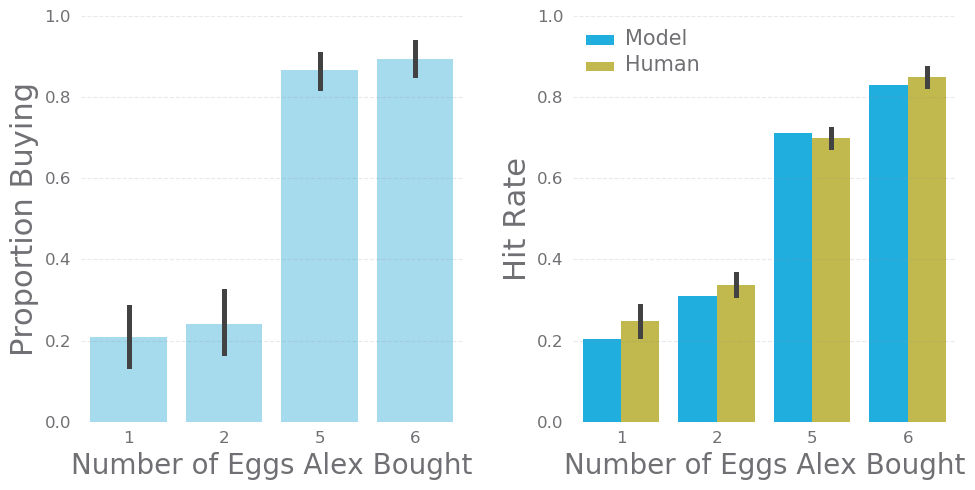
\includegraphics[width=\linewidth]{exp1.png}
  \caption{Results from Experiment 1: (Left) The proportion of participants deciding to buy a new egg as a function of the number of eggs Alex bought. (Right) Hit rates of robot chickens predicted by the model vs. inferred by participants. (Error bars indicate the 95\% confidence intervals.)}
  \label{fig:exp1}
\end{figure}

The central question that inspired this research is whether people would still reproduce observed disparities even without existing stereotypes. In Experiment 1, this question translates to whether participants' purchase decisions were influence by Alex's check rates. From Figure \ref{fig:exp1} (left), it's obvious that far more participants chose to buy a new egg when Alex bought 5 or 6 eggs compared to only 1 or 2. To test this observation more rigorously, we fit a generalized linear mixed model (GLMM) using the R package \texttt{lme4} \citep*{bates2015fitting} with participants' purchase decisions as the outcome variable, the number of eggs Alex bought as the fixed effect, as well as random intercepts and slopes for participants and trials\footnote{Here we implemented \texttt{lme4} models in Python via \texttt{rpy2} to keep in the same environment. The formula for the full model was: \texttt{buy $\sim$ checked + (1 {\textbar} participant) + (1 {\textbar} trial)}.}. Consistent our observation, with each additional egg Alex bought, the odds ratio for participants buying an egg increased by 2.36, which was significantly higher than chance, Wald's $\chi^2$ = 14.03, $p = .00018$. 

Were participants ``mindlessly'' copying Alex's sampling behavior or did they use it to infer robot chickens' hit rates in a ``rational'' way? To answer this question, we examined whether participants' hit rate inferences can be captured by a NUC model. First of all, we estimated parameters values in Equation \ref{eq3} to be $\beta_0 = -2.56$ and $\beta_1 = .98$ using the Python library \texttt{PyMC3} \citep*{salvatier2016probabilistic} based on participants' inferred hit rates and purchase decisions. Then we implemented a ``check rate only'' NUC model to predict how people should infer each chicken's hit rate from Alex's check rate and compared model predictions against participants' actual inferences. As you can see in Figure \ref{fig:exp1} (right), this NUC model captured all the qualitative trends across all trial types. Model predictions were strongly correlated with human responses, Pearson's $r = .79$, $p < .001$. 

\subsection{Discussions} 
Before playing the Golden Ticket, participants had no expectation for each robot chicken's hit rate. Yet, after watching a knowledgeable, utility-maximizing agent Alex playing the game, participants quickly followed their lead, buying more eggs from chickens that Alex was more likely to buy from. This result shows that participants ended up reproducing observed disparities in check rates without having prior stereotypes of chickens' hit rates. At least when explicitly asked to, participants could do more than just blindly copying Alex's sampling behavior: Each chicken's hit rate that they inferred from Alex's check rate closely matched the prediction generated by a simple Na\"ive Utility Calculus model. Perhaps through a similar inferential process, a na\"ive observer of police encounters may conclude that groups under heavier scrutiny have higher crime rates and will check members from these groups more often when given the opportunity.

What if groups checked more often have the same or even lower hit rates? One of the most striking and informative findings from the Oakland police stop data is that African Americans who were stopped far more often than other races were no more likely to carry contraband. If people trust a knowledgeable, utility-maximizing agent blindly, they may disregard this new hit rate information as a ``fluke''. It's also possible that they ignore the agent's sampling behavior and solely focus on observed hit rates. Alternatively, people may consider both the hit rates and the check rates in the sample to infer group hit rates. To examine these possibilities, we conducted Experiment 2 where Alex opened the purchased eggs to reveal which ones had tickets and which ones were empty. 

\section{Experiment 2}

\subsection{Methods}

\subsubsection{Participants}
Sixty-seven adult residents of the United States (mean age = 36.9 years) participated in Experiment 2 through Amazon Mechanical Turk. To participate, one must have a past acceptance rate of 95\% or above and not have taken part in Experiment 1. Another 30 participants were excluded for failing any of the five instruction check questions. All participants gave informed consent prior to the study and were paid \$2 for about 15-20 minutes of their time. 

\subsubsection{Procedure} 
The procedure for Experiment 2 was identical to that for Experiment 1, except that Alex opened the eggs they bought in the end to reveal which ones had tickets and which ones were empty. There were 12 unique combinations of how many eggs had tickets out of how many eggs Alex bought. Of these, there were 6 critical trials where Alex bought most or all eggs but most or all were empty (\underline{0 or 1 out of 6} eggs or \underline{0 or 1 out of 5} eggs had tickets) or few eggs but all had tickets (\underline{1 out of 1} egg or \underline{2 out 2} eggs had tickets). In case participants suspected that Alex was misleading or not actually knowledgeable, we added 6 ``filler'' trials where Alex bought most or all eggs and most or all had tickets (\underline{5 or 6 out of 6} eggs or \underline{4 or 5 out of 5} eggs had tickets) or few eggs and none had tickets (\underline{0 out of 1} egg or \underline{0 out 2} eggs had tickets). The order of presentation was randomized across participants.

\subsection{Results} 
\begin{figure}[t]
  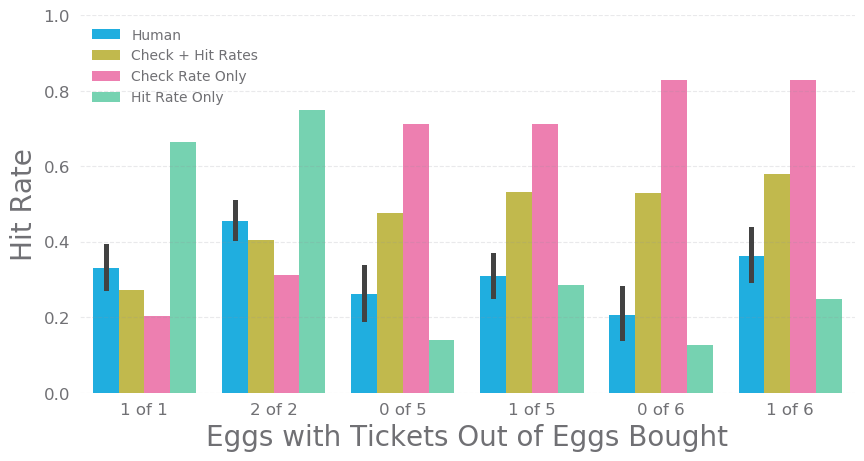
\includegraphics[width=\linewidth]{exp2.png}
  \caption{Results from Experiment 2: Hit rates of robot chickens predicted by three models (``check + hit rates'', ``check rate only'', ``hit rate only'') vs. inferred by participants. (Error bars indicate the 95\% confidence intervals.)}
  \label{fig:exp2}
\end{figure}

After observing both the check rate and the hit rate in an egg sample, how did participants infer the chicken's true hit rate? We created the three models to capture three hypotheses (Figure \ref{fig:models}): 1) a NUC model inferring hit rates from both observed check rates and hit rates (``check + hit rates"), 2) another NUC model only inferring from observed check rates (``check rate only"), and 3) a non-NUC ``hit rate only'' model.

Based on participants' inferred hit rates and purchase decisions, we estimated the parameter values in Equation \ref{eq2} to be $\beta_0 = -2.79$ and $\beta_1 = 1.10$. The we implemented the above models using the estimates (with the exception of the ``hit rate only'' model, which doesn't require these parameters). To see which model resembled human performance the most, we used the root mean square error\footnote{In this case, $\mathrm{RMSE} = \sqrt{(\frac{1}{n})\sum_{i=1}^{n}(\theta_{m_{i}} - \theta_{h_{i}})^{2}}$, where $n$ is the number of participants and $\theta_{m}$ and $\theta_{h}$ are hit rates predicted by a model and inferred by participants, respectively.} (RMSE) to measure the dissimilarity between model predictions and human inferences. Lower RMSE indicates better model fit. As it turned out, the ``check rate only'' model's predictions strayed furthest away from human inferences (RMSE = .37) whereas the ``check + hit rates'' model and the ``hit rate only'' model (RMSE = .27 and RMSE = .26, respectively) performed similarly. 

Figure \ref{fig:exp2} compared model predictions with human inferences across 6 critical trials\footnote{Models made similar predictions on non-critical trials. In the interest of space and model comparison, we didn't plot these trials.} where observed hit rates and check rates were at odds with each other (i.e., when one was high, then the other was low). Not a single model captured all the qualitative trends across all trial types. Among the three, the ``check rate only'' model was the least accurate one, grossly overestimating hit rates when Alex bought many eggs and underestimating when few. The ``check + hit rates'' model and the ``hit rate only'' model both captured part of the trends: When Alex bought just few eggs but all had tickets, the ``check + hit rates'' model was the most accurate; when Alex bought bought many eggs but few had tickets, the ``hit rate only'' model performed most similarly to humans.

\subsection{Discussions} 
All in all, no model captured participants' hit rate inferences exactly when both check rate and hit rate information was available. Why did the ``check + hit rates'' model and the ``hit rate only'' model each predict some but not all of the patterns? One possibility was that hit rate information was \emph{more salient} than check rate information. The last four conditions shown in Figure \ref{fig:exp2} provided strong evidence for both high check rates (e.g., 6 bought out of 6 available) and low hit rates (e.g., 0 with a ticket out of 6 bought). When evidence for both was more or less equally strong, participants seemed to value the evidence of low hit rates over that of high check rates. In the first two conditions, there was strong evidence for low check rates (e.g., 1 bought out 6 available) but only weak evidence for high hit rates (e.g., 1 with a ticket out of 1 bought). It seemed only when hit rate information lacked strength did participants put emphasis on check rate information. 

To test whether participants placed a higher weight on hit rate information, we fit a linear regression model using predictions generated by the ``hit rate only'' model and the ``check rate only'' model to predict human inferences. The estimated coefficient of the former (0.64) was greater than that of the latter (0.42), suggesting that participants may indeed have relied more on observed hit rates than check rates. 

Of course, it's possible that some participants mostly relied on check rates and some on hit rates. In future research, we could use latent mixture models or similar techniques to identify subgroups and capture each subgroup's behavior.

\section{General Discussion}
Racial disparities have deep roots in societies around the world. Unfortunately, awareness doesn't always translate into the desire to end disparities. When reminded of racial disparities in prison, people became even more supportive of harsh criminal law that helped create them in the first place \citep[e.g.,][]{hetey2014racial,hetey2018numbers}. Aside from stereotypic associations linking Blacks with crime, we argue that rational inference alone based on Na\"ive Utility Calculus (NUC) \citep{jara2016naive} can also reproduce disparities: If people believe police officers are knowledgeable about different races' ``true crime rates'' and act to maximize expected utilities (expected rewards of catching criminals relative to the total costs of checking), they may think groups under heavier scrutiny have higher crime rates and target them as well. 

This is what we found in Experiment 1 when only check rates were available. To simulate police encounters without evoking stereotypes, we created a ``Golden Ticket'' game where robot chickens (``groups'') lay eggs (``groups members'') that may or may not have golden tickets (``crime'') inside. Each ticket can be redeemed for a prize but each egg costs a token. Participants watched a knowledgeable, utility-maximizing agent Alex play a series of chickens, after which they were asked to infer each chicken's ``hit rate'' and decide whether or not to buy a new egg from it. While participants had no prior stereotypes linking certain chickens with high or low hit rates, they reproduced disparities in Alex's sampling behavior nonetheless: The more eggs Alex bought, the more likely participants would buy from the same chicken. To show that participants were not copying without thinking, we asked them to infer each chicken's hit rate and their inferences closely matched a rational NUC model. Once again, these suggest that merely exposing people to disparities without addressing the underlying causes may well backfire. In Experiment 2, participants got to observe hit rates in the samples: Alex opened the eggs they bought in the end to reveal which ones had tickets and which ones didn't. Participants seemed to rely more on this new hit rate information than the agent's sampling behavior. Given strong evidence for high check rates (e.g., Alex bought 6 eggs out of 6) and low hit rates (e.g., 0 out of 6 eggs had tickets), participants expected true hit rates to be low. This was captured by a "hit rate only" that ignored check rates. When the evidence was strong for low check rates (e.g., bought 1 out of 6) but weak for high hit rates (e.g., 1 out of 1 egg had a ticket), participants inferred the true hit rates to be in a middling range. This inference was captured by the ``check + hit rates'' model.

A number of reasons may explain why participants seemed to value hit rate information more. Perhaps assuming that observed hit rates are equal to true hit rates takes less mental effort than decoding Alex's motivation (\emph{``They wouldn't have bought so many eggs if this chicken weren't profitable.''}). It could also be that participants doubted Alex's knowledge after a few ``failures'' (\emph{``Maybe they haven't played with this one before?''}), even though they were reminded that Alex knew all chickens' hit rates really well. In follow-up studies, we can ask participants to rate Alex's credibility throughout the experiment to examine these hypotheses. Regardless of the underlying mechanism, findings in Experiment 2 suggested a way to fight disparities: Showing that groups targeted by the police are not necessarily more prone to crime may help people re-evaluate the true crime rates more objectively. 

\subsection{Future directions}
Oftentimes, we don't just see one police officer repeatedly targeting certain groups but many across the nation targeting the same groups. To a na\"ive observer, consensus may be an even stronger indicator of ``ground truth''. In future work, we wish to look at whether hit rate information becomes less powerful when it goes against the consensus among multiple rational agents. Also, we used non-social groups in this study but it's likely that people reason about social groups differently. We will investigate this possibility in the future.

\section{Acknowledgment}
We thank Julian Jara-Ettinger, Tomer Ullman, Steve Piantadosi, Mahesh Srinivasan, the Berkeley Early Learning Lab, and four anonymous reviewers for their generous suggestions and thoughtful discussions that inspired and shaped this work.

\vskip 3mm

\fbox{
  \begin{minipage}{20em}
  \centering
  Data and code used in this work are available at \href{https://github.com/Yuan-Meng/PISG}{\texttt{https://github.com/Yuan-Meng/PISG}}
  \end{minipage}
  }

\bibliographystyle{apacite}
\renewcommand\bibliographytypesize{\footnotesize}
\setlength{\bibleftmargin}{.125in}
\setlength{\bibindent}{-\bibleftmargin}

\bibliography{PISG}

\nocite{liu19}

\end{document}
